\documentclass{article}

\usepackage[utf8]{inputenc}
\usepackage[T1]{fontenc}
\usepackage{geometry}
\usepackage{xcolor}
\usepackage{graphicx}
\usepackage{subcaption}
\usepackage{verbatim}
\usepackage{amsmath,amssymb}
\usepackage{amstext}
\usepackage{amsthm}
\usepackage{steinmetz}
\usepackage{stackrel}
\usepackage{mathtools}
\newcommand{\angstrom}{\text{\normalfont\AA}}

\geometry{a4paper}

\usepackage[english]{babel}
\frenchspacing

\title{Report: adder and subtractor}
\author{Lorenzo Ramella, Alessandro Matteo Rossi, Marco Tambini}
\date{\today}

\begin{document}
\maketitle

\tableofcontents

\section{Basics concepts}

To make calculations, a circuit needs to be able to perform logical operations. In particular, we usually use boolean algebra in digital electronics. 

\vspace{3mm}

To be able to create a circuit like this, first of all, we need to define the various components.
The number 0 and 1 need to be properties of an electrical circuit that can be "moved" and they can be realized using voltage. We can assign the number 0 to a low voltage and the number 1 to a high voltage. 

\vspace{3mm}

For example, if we define $0\,\textrm{V}$ as low, negative or 0 and $5\,\textrm{V}$ as high, positive or 1, we can define a threshold voltage exactly in the middle, so that any voltage under $2.5\,\textrm{V}$ will be considered 0, and any voltage above it will be considered 1.

\vspace{3mm}

Once 1 and 0 are defined, we need to define the operations that can be performed:

\begin{itemize}
\item $"!"$ is the negation, and it can be represented by a NOT gate.
\item $"+"$ is the addition, and it can be represented by an OR gate.
\item $"*"$ is the multiplication, and it can be represented by an AND gate.
\end{itemize}

\section{Logic gates}

When we talk about a logic gate, we are describing a circuit that can take a certain number of inputs and gives a single output, depending on the input received. The output needs to be readable by another logic gate of the same family.

\vspace{3mm}

The main logic gates are the following, represented with their circuital symbol in figure \ref{LogicGates}.

\begin{figure}[h!]

    \centering
    \begin{subfigure}{.4\textwidth}
        \centering
        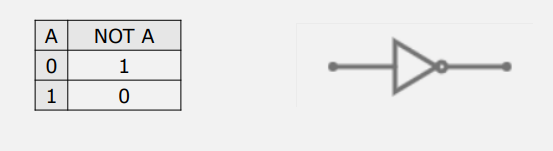
\includegraphics[width=\linewidth]{IM_NOT.PNG}
        \caption{NOT gate}
        \label{NOT}
    \end{subfigure}
    \hfill
    \begin{subfigure}{.4\textwidth}
        \centering
        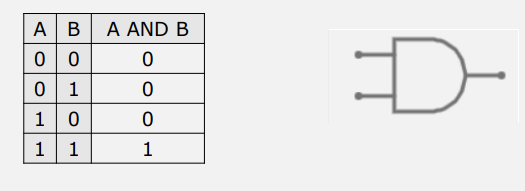
\includegraphics[width=\linewidth]{IM_AND.PNG}
        \caption{AND gate}
        \label{AND}        
    \end{subfigure}
    
    \centering
    \begin{subfigure}{.4\textwidth}
        \centering
        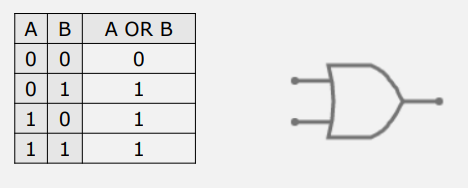
\includegraphics[width=\linewidth]{IM_OR.PNG}
        \caption{OR gate}
        \label{OR}
    \end{subfigure}
    \hfill
    \begin{subfigure}{.4\textwidth}
        \centering
        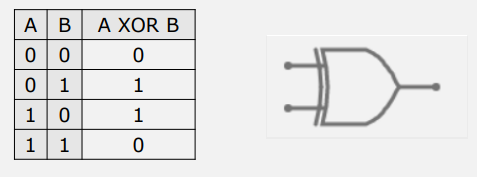
\includegraphics[width=\linewidth]{IM_XOR.PNG}
        \caption{XOR gate}
        \label{XOR}        
    \end{subfigure}
    
    \centering
    \begin{subfigure}{.4\textwidth}
        \centering
        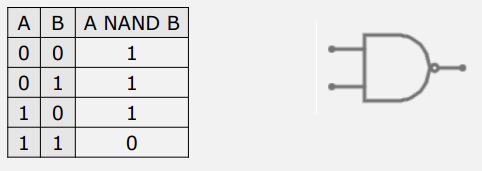
\includegraphics[width=\linewidth]{IM_NAND.PNG}
        \caption{NAND gate}
        \label{NAND}
    \end{subfigure}
    \hfill
    \begin{subfigure}{.4\textwidth}
        \centering
        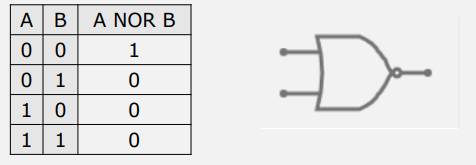
\includegraphics[width=\linewidth]{IM_NOR.PNG}
        \caption{NOR gate}
        \label{NOR}        
    \end{subfigure}
    
    \centering
    \begin{subfigure}{.4\textwidth}
        \centering
        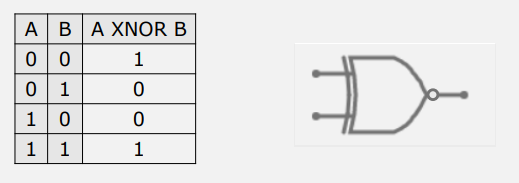
\includegraphics[width=\linewidth]{IM_XNOR.PNG}
        \caption{XNOR gate}
        \label{XNOR}
    \end{subfigure}

\caption{Image of the main logic gates used in digital electronics}
\label{LogicGates}
\end{figure}


\subsection{N-MOS}

In order to create these logic gates, we need to know how to use a MOSFET. For this project we used N-MOS transistors only.

\vspace{3mm}

The N-MOS is a transistor that gets as input a gate voltage, a drain voltage, a source voltage and a body voltage. In most cases the source and the body are internally connected, since the body needs to be at the lowest voltage and the source is usually grounded.

\vspace{3mm}

When a positive voltage is applied between the drain and source, a deplition layer that blocks the current flow is formed. 
If we then start applying a positive voltage between gate and body, the electrons will start "balancing" the gaps in the P substrate, but the current will still be zero.

\vspace{3mm}

After $V_{GS}$ (the potential difference among gate and source) overcomes a certain threshold voltage, the current will start to flow from drain to source. At the beginning of this flow, the ratio between the current and $V_{DS}$ (the potential difference among drain and source) is linear but, when $V_{DS}$ becomes big enough, the function becomes almost constant (see figure \ref{NMOS_Function}) and we find ourself in the saturation region.

\begin{figure}[h]
    \centering
    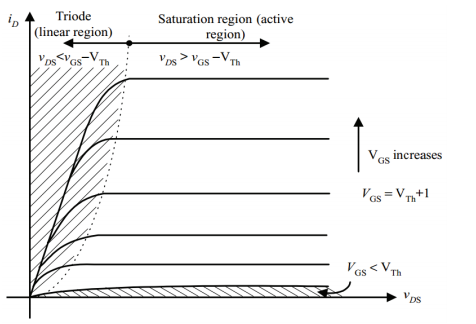
\includegraphics[scale=.65]{IM_NMOS_Function.png}
    \caption{Graph of the I-V N-MOS function}
    \label{NMOS_Function}
\end{figure}

\vspace{3mm}

We do not need to distinguish linear section and saturation section, as we will check only the voltage at the drain of the N-MOS for our gate. The threshold voltage is different for every transistor, and it usually is within the range $0.5\,\textrm{V} - 5\,\textrm{V}$. The transistor we used is the $IRF822$, whose threshold voltage has been measured in lab, and it is approximately %nV
. We decided to use $5\,\textrm{V}$ for $V_{GS}$ to make input and output approximately the same, as we will see later.



\subsection{NOT gate}

The easiest logic gate to realize is the NOT gate. We remember that the NOT gate negates the only input it receives. We need a high enough resistance and one N-MOS (as represented in figure \ref{NOT_N-MOS}) to realize it.
\clearpage
\begin{figure}[h]
    \centering
    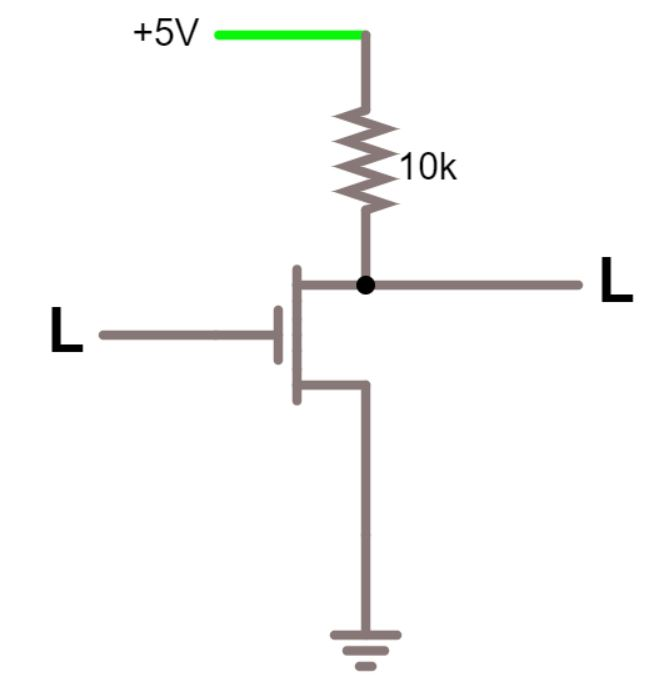
\includegraphics[scale=0.3]{IM_NOT_NMOS.JPG}
    \caption{NOT logic gate realized using a N-MOS and a resistor}
    \label{NOT_N-MOS}
\end{figure}

When the input is 0, the N-MOS will not let the current flow and, thanks to Ohm First Law, we know that the voltage drop across the resistor should be 0, so we get the same supply voltage. The read output will be around $5\,\textrm{V}$, so we get a 1 as output.

\vspace{3mm}

When the input is 1, the N-MOS will let the current flow with a small resistance value. Since there is a higher resistance before the N-MOS, almost all the voltage drop will occur on the previous one, and the drain will be almost zero. The read output will be around $0\,\textrm{V}$, so we get a 0 output.

\vspace{3mm}

With this configuration the signal will not be properly negated for high frequencies, and it will be like in the last picture in figure \ref{ResistiveInverter} (it will never reach a 1 state).

A possible solution consists of a combination of N-MOS and P-MOS but, since our calculator does not have to work at such high frequencies, we dismissed this problem.

\begin{figure}[h]
    \centering
    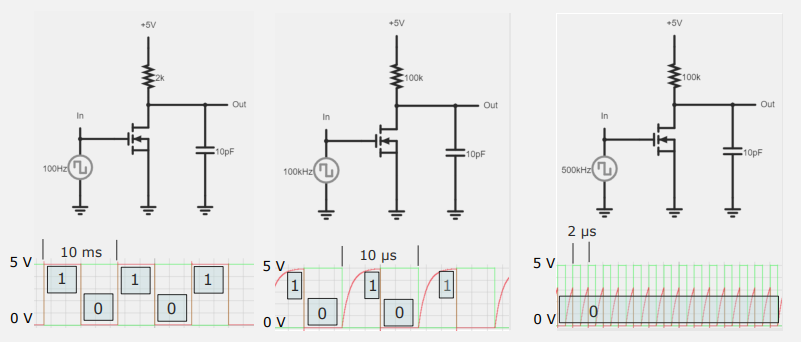
\includegraphics[scale=0.6]{IM_inverter_esa.PNG}
    \caption{Inverter N-MOS circuit with a resistive load}
    \label{ResistiveInverter}
\end{figure}

For the immage of the NOT gate and some result we got in lab check the end of the report at %number of appendix chapter subsection not gate


\clearpage
\subsection{NOR gate}

Once we created the NOT gate, we proceeded to realize the NOR gate since, as we will explain later in Section \ref{OtherGates}, the NOR and the NAND gate are both functional complete.

\vspace{1mm}

The NOR gate is composed, as seen in figure \ref{NOR_N-MOS}, by two NOT gates short-circuited at their output.

\begin{figure}[h]
    \centering
    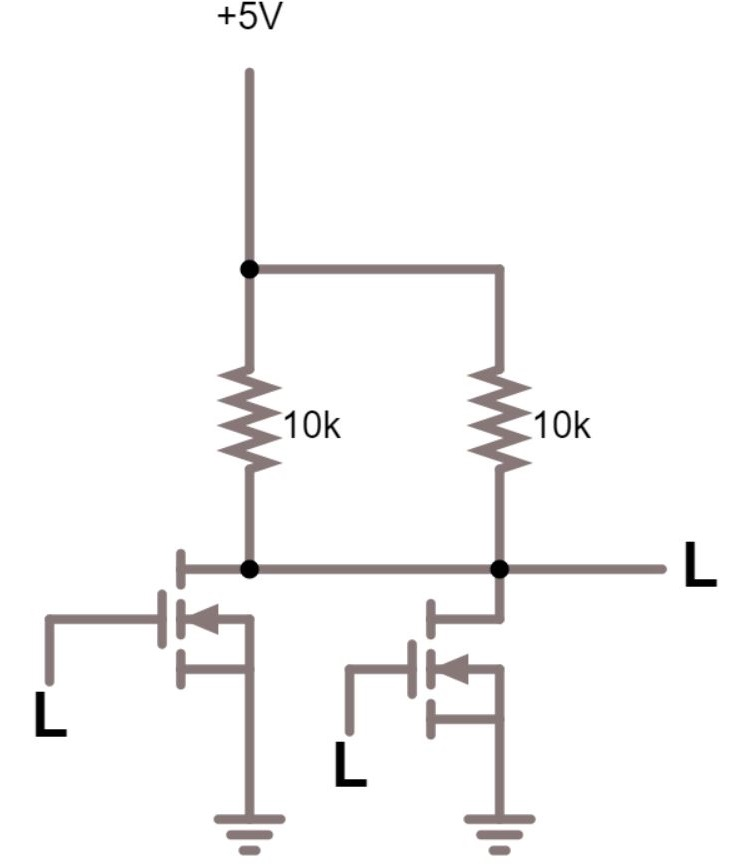
\includegraphics[scale=.3]{IM_NOR_NMOS.JPG}
    \caption{NOR logic gate realized using two short-circuited NOT gates}
    \label{NOR_N-MOS}
\end{figure}

When both inputs are 0, the two N-MOS will not let any current pass and, just like in the NOT gate, the output will be 1.

\vspace{1mm}

When one or both inputs are 1 the N-MOS will let the current flow and there will be a voltage drop across the resistor. So the output will be 0.

\vspace{1mm}

The role of the short circuit is ensuring that whether an input is positive, the current will pass through the "open" N-MOS.

\vspace{3mm}

For the immage of the NOR gate and some result we got in lab check the end of the report at %number of appendix chapter subsection nor gate

\subsection{NAND gate}

As we said for the NOR gate, the NAND gate is also functional complete. But it can be created without the shortcircuit and without one of the resistors needed by the NOR gate, so it is slightly cheaper. 

\vspace{3mm}

The NAND gate is realized with a series resistor followed by two N-MOS, where the source of the first is plugged in the drain of the second, as seen in figure \ref{NAND_NMOS}.

\begin{figure}[h]
    \centering
    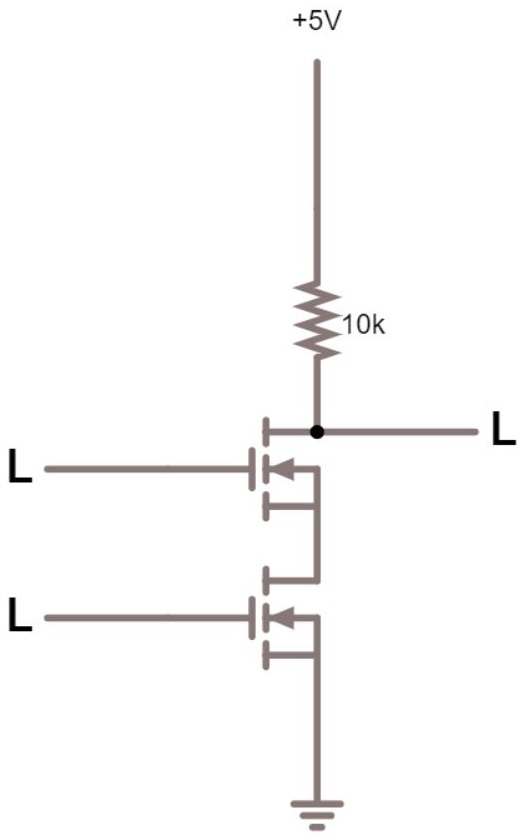
\includegraphics[scale=.25]{IM_NAND_NMOS.JPG}
    \caption{NAND gate realized with one resistor and two N-MOS transistors}
    \label{NAND_NMOS}
\end{figure}

\vspace{3mm}

When both inputs are 1, the current will be able to flow and the output will be 0.

\vspace{1mm}

When one of the inputs is 0, one of the N-MOS will be "closed" and, since the current cannot pass, the output will be 1.

\vspace{3mm}

For the immage of the NAND gate and some result we got in lab check the end of the report at %number of appendix chapter subsection nand gate



\subsection{Other logic gates} \label{OtherGates}

Being functional complete means that a single logic gate can be the only component in a circuit, and that circuit will be equivalent to any other logic gate. NAND and NOR gates have this property (see figure \ref{NAND_allpowerful} and \ref{NOR_allpowerful} in appendix).

\vspace{3mm}

The only gates needed for the calculator are shown in figure \ref{UsefulGates}, and they are: 

\begin{itemize}
\item The AND gate, made by the NAND gate, where the output is negated by a NOT.
\item The OR gate, made by the NOR gate, where the output is negated by a NOT.
\item The XOR gate, made by four NAND gates as shown in figure \ref{XOR_NANDs}
\end{itemize}

\begin{figure}[h]
    \centering
    \begin{subfigure}{.49\textwidth}
        \centering
        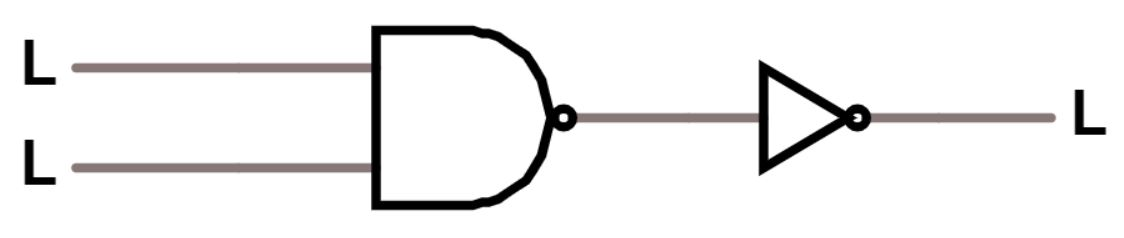
\includegraphics[scale=.3]{IM_AND_LOGIC.JPG}
        \caption{AND gate built using a negated NAND gate}
    \end{subfigure}
    \hfill
    \begin{subfigure}{.49\textwidth}
        \centering
        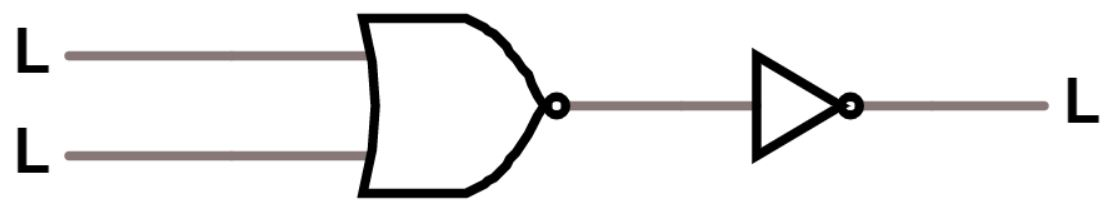
\includegraphics[scale=.3]{IM_OR_LOGIC.JPG}
        \caption{OR gate built using a negated NOR gate}       
    \end{subfigure}
    \vspace{2mm}
    \begin{subfigure}{\textwidth}
        \centering
        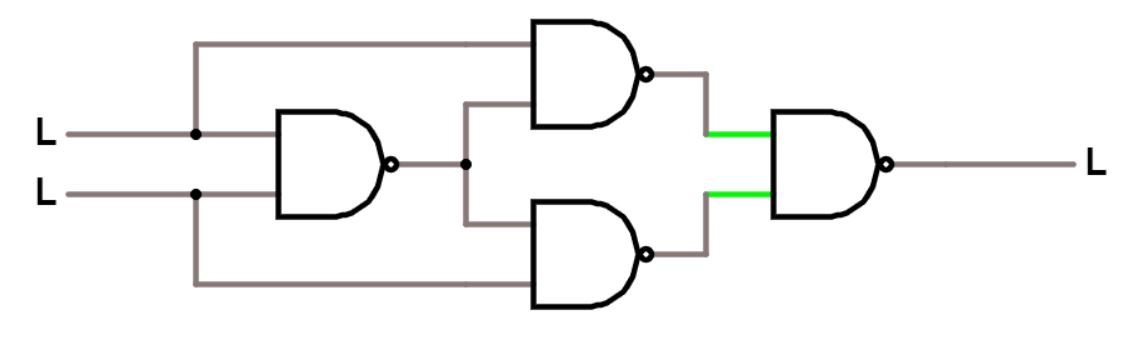
\includegraphics[scale=.3]{IM_XOR_LOGIC.JPG}
        \caption{XOR gate built using a four NAND gates}     
        \label{XOR_NANDs}     
    \end{subfigure}
    \caption{The logic gates used in the calculator}
    \label{UsefulGates}
\end{figure}
\clearpage
\subsection{Bistable circuit}

For the 16-bit calculator, that will be discussed in section \ref{SimulatedCalculator}, we also needed to be able to store information.

\vspace{1mm}

This means that we need a component that will work as memory. It has to be able to get an input and keep it saved as long as necessary, even if the input signal has already expired. Since the memory has to be both writable and readable, it needs a second input line to clear it.

\vspace{3mm}

The circuit that corresponds to the memory we need is the bistable circuit, also known as flip-flop (shown in figure \ref{FlipFlop}).

\begin{figure}[h]
    \centering
    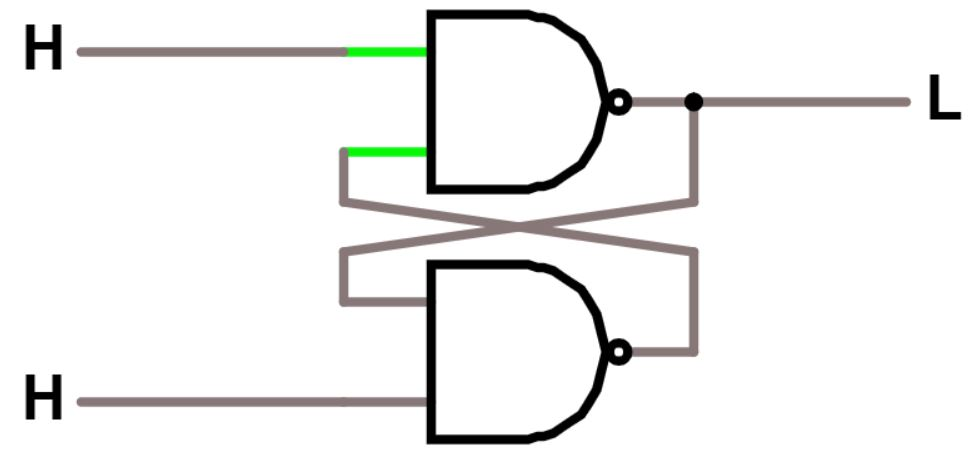
\includegraphics[scale=.3]{IM_FlipFlop}
    \caption{The circuit used to create a flip-flop memory unit}
    \label{FlipFlop}   
\end{figure}

The flip-flop can be created by both NOR gates and NAND gates but, since the NAND gates are cheaper, we decided to use those. This meant that the input has to be negated in order to work properly. Flip-flop truth table can be found in table \ref{FlipFlopTT}.


\begin{table}[h]
\centering
\begin{tabular}{ | c | c  c  c | c  c |}
\hline
 \# & $Set$ & $Clear$ & $Old Q$ & $New Q$ & $New Q'$\\
\hline
 \ 1 & 0 & 0 & 0 & 1 & 1 \\ 
 \ 2 & 0 & 0 & 1 & 1 & 1 \\
\hline 
 \ 3 & 0 & 1 & 0 & 1 & 0 \\ 
 \ 4 & 0 & 1 & 1 & 1 & 0 \\ 
 \ 5 & 1 & 0 & 0 & 0 & 1 \\
 \ 6 & 1 & 0 & 1 & 0 & 1 \\
\hline
 \ 7 & 1 & 1 & 0 & 0 & 1 \\
 \ 8 & 1 & 1 & 1 & 1 & 0 \\ 
\hline
\end{tabular}
\caption{Flip-flop truth table. Please note that the first two rows are not ideal for the storage of data, as $Q$ and $Q'$ have the same value. Rows 3-6 represent the moment when an input is given, whereas 7 and 8 is when data is stored.}
\label{FlipFlopTT}
\end{table}


\clearpage

\section{16-bit calculator} \label{SimulatedCalculator}



\subsection{Input with 16-bit}

Our goal is to create a 16-bit calculator. It has to receive 16 bits as input and that produces 17 output bits (the 17th is the sign bit).

\vspace{3mm}

One of the problems that arise when we want to use such a big memory space is the increasement in complexity; this makes the circuit more expensive and also takes a lot of physical space, that could be used for other purposes. In a small scale, we could use a 2-bit priority encoder, but, for our project, it would be unpractical and unnecessarily harder.

\vspace{3mm}

Another problem regarding the priority encoder, is that this component would require more physical space. We would need an input line for every single number we could insert. Considering that the possible inputs are all the natural numbers in the interval $[0,2^{16})$, we would need $2^{16}$ input lines.

\vspace{3mm}

To solve both problems we decided to use a keyboard. It takes the input through some buttons, instead of the levers we used in the laboratory. This method solved both the problem with the number of inputs and the problem of the complexity of the decoder.



\subsection{Keyboard}

The keyboard part connects a point at high voltage to the rest of the circuits. It is composed by: 

\begin{itemize}
    \item 10 buttons for the digits from 0 to 9;
    \item An addition button labeled $+$;
    \item A subtraction button labeled $-$;
    \item A button to have the result displayed, labeled $=$;
    \item A clear button that resets the entire circuit.
\end{itemize}

\begin{figure}[h]
    \centering
    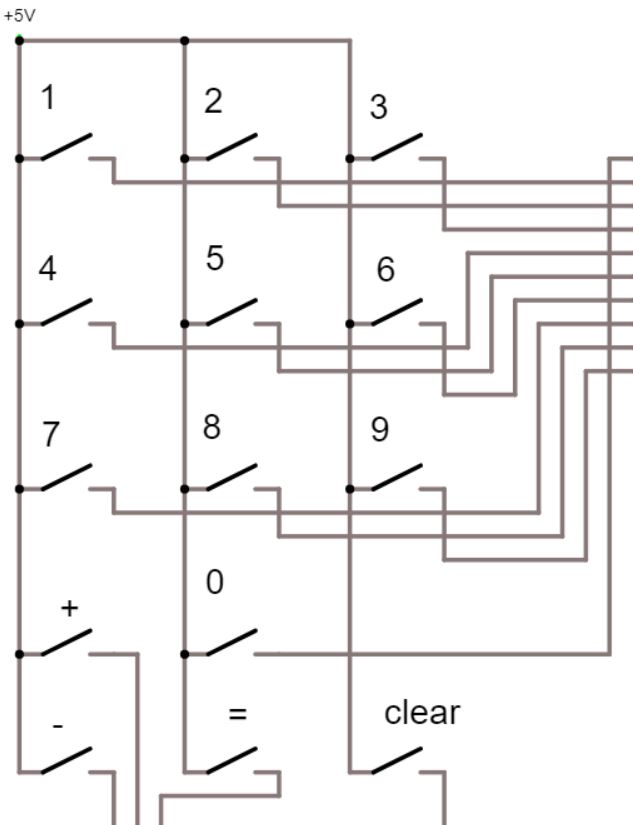
\includegraphics[scale=.3]{IM_Keyboard}
    \caption{Picture of the simulated circuited keyboard}
    \label{Keybaord}
\end{figure}

\clearpage

\subsection{4-bit encoder}
The first part of our encoder is a 4-bit encoder, without priority. 

\begin{figure}[h]
    \centering
    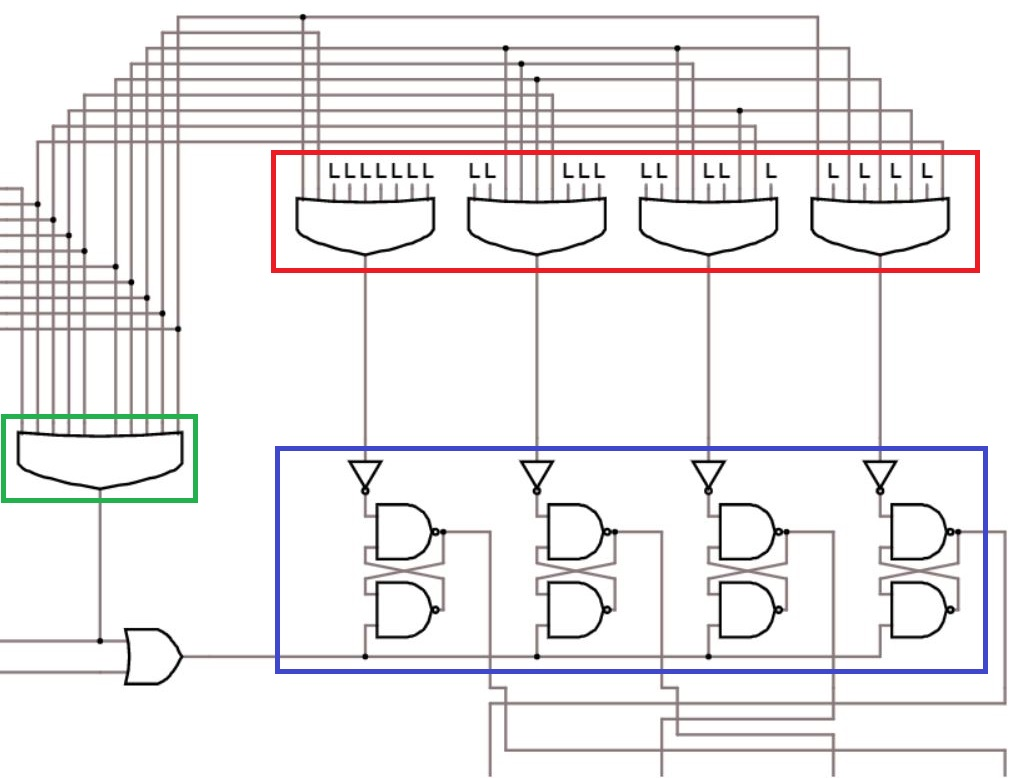
\includegraphics[scale=.35]{IM_4BitEncoder.JPG}
    \caption{4-bit encoder}
    \label{encoder}
\end{figure}

As you can see in figure \ref{encoder} this part can be split in three different sections:

\begin{itemize}
    \item The red part is a 4-bit encoder without priority. As we were saying in the paragraph above, the advantage of using a keyboard is that we will, under normal condition, only get 1 input at a time making a priority encoder useless. The encoder works by checking, with an OR gate, which bits the inserted number activates.
    
    \vspace{1mm}

    For example, if we press the button "6" the binary input will be $0110$, so only the second and the third bit will be activated.

    \item The green part is an OR gate connected to all the input lines, in order to check whether a button corresponding to a number is pressed. This choice has been made because if 0 was pressed, it should not result in any binary input, but it would be read as the number $10$. 

    \item The blue part is a small "flash memory", which gets cleared when the input button is no longer pressed. 
            
        This part, whose task will be discussed in the next subsection, is a simple "security" method useful to ensure that the inputs arrive correctly to the next memory. This part could be removed if the circuit timing was perfect, but we preferred to keep it to ensure no problem would arise.    
\end{itemize}


\subsection{Memory and successive inputs}

This part allows the circuit to receive that make possible to get consecutive inputs, and it is composed by two memories and two full adders. 

In this section the input gets stored and, after a new button is pressed, the stored number is multiplied by 10 and then added to the new input. By doing this we can obtain every number within the memory limit.

It is important to point out that this part works by using the concepts of "rising edge", where the input passes from a low state to a high one, and "falling edge", where the input changes from high to low. Using this concept it is possible to process a single input in two phases.

\begin{figure}[h]
    \centering
    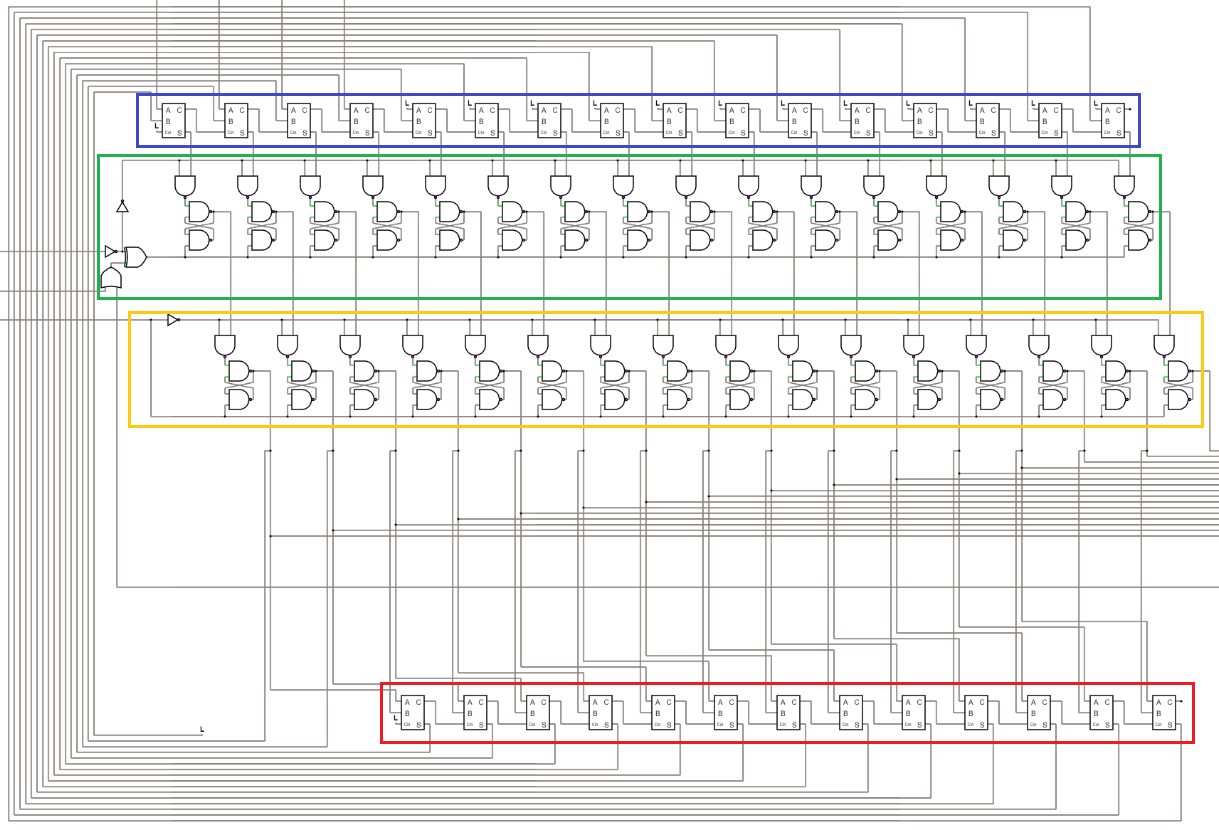
\includegraphics[scale=.55]{IM_Converter.PNG}
    \caption{}
    \label{Converter}
\end{figure}


\subsubsection{Rising edge}

When the first button is pressed, the circuit is in a state of "rising edge". In this moment the first memory horizontal wire, that goes to all the NANDs of the second memory (highlighted in yellow in figure \ref{Converter}), switches to low to prevent the NAND from letting any signal pass from the first to the second memory.

\vspace{1mm}

The second wire involved is the horizontal one under the first memory (highlighted in green), that also turns off; this line is responsible for clearing the memory when it switches from high to low.

\vspace{1mm}

After a little while, the last wire that changes is the one on top of the first memory, that allows a new input to be memorized in the cleared memory.

\vspace{3mm}

It's important to note that, during the data storage, the reset button is in a low state, since it cleared the memory right before the storage of new data.

\vspace{1mm}
%non ho capito un cazzo di fino al prossimo vspace
This statement don't pose problem when the input is 0 since we find ourself in the case 5 or 6 of the flip-flop truth table (table \ref{FlipFlopTT}) and, as you can see, the output is 0. 

The problem arise when the input data is 1 since we find ourself in case 1 or 2 where the two input are 0; as we can see in the truth table both output are set at 1.

After one of the two input switch from low to high the flip-flop return in a normal state; what we want is to go from the state above to the state 4 of the table of truth; this mean that, as long as the first line to return to high is the one for the reset, we see no problem.

\vspace{3mm}

The problem we just described has been solved in the simulated calculator by using the delay given from the logic gates. In reality, this could be a problem since this relies on physical properties that could depend from temperature, making this kind of timing, whether applied to a real circuit, not as precise as in the simulator.

\vspace{1mm}

The timing problem also includes the fact that the operation on the second memory should be done before the one on the first memory. In our circuit the first memory delay is performed by the clearing part on the low left side of the first memory. % non si capisce bene

\vspace{1mm}

Another possible solution could be using an external clock to define when the action should be performed but, in order to keep our simulated circuit as easy as possible, we decided to simply address the problem in this report.




\subsubsection{Falling edge}

After the button is released the circuit finds itself in falling edge phase.

\vspace{3mm}

The process is similar to the previous one: the first wire to change this time is the one below the second memory. Its task is the memory reset, like the one in the first memory. After this, the wire on top of the second memory change its state to allow the last one (CHE SAREBBE?) to store information coming from the first memory.

The last connection that switches is, as before, the horizontal one on top of the first memory. It switches from high to low and prevents any further memory modification.

\vspace{3mm}

The problem described at the end of the rising edge is, in fact, a problem that begins during the rising edge and ends at the falling edge. Since the first memory works during the rising edge phase, and the second one works during the falling edge phase, the second memory will suffer the same problem, and so it will have the same possible solution explained before.


\subsubsection{Multiplication}

The full adders work between the falling edge and the rising edge.

\vspace{3mm}

The second full adder, highlighted in red, is the one responsible of multiplying 10 to the previous number and, as already said, it works among falling edge and rising edge.

\vspace{3mm}

To do a multiplication in binary you need to shift the number as much as the bit of the multiplier and add all the result. For example let's take $6 \cdot 10$, writing it in binary we obtain 
$0110 \cdot 1010$. if we subdivide the multiplication if $0110 \cdot 1000$ and $0110 \cdot 0010$ we can simply shift the number. 
after this we add the two result $101000 + 001010 = 110010$ and the result that we obtain corresponds with 60 in decimal form. %riformulare

\vspace{3mm}

To do this operation we simply let the input go to the second and fourth entrance of the adder and take in output the result multiplied by 10. Since the multiplier is 10 we can see that the first bit of the result will always be low and that the first three number of the result don't need any addition so we can directly take result without passing by a full adder. %eh?


\subsubsection{Adder}

The first adder, highlighted in blue, has the duty of adding the previous number, multiplied by 10, to the new number in input. This second adder works between the rising edge and the falling edge. 



\subsection{Sign bit}

To do the subtraction we could have used the full subtractor, but we decided to use the addition between positive and negative number in binary. To do the subtraction we needed a way to read whether the second number was positive or negative. As visible in figure \ref{SignBit} we simply used a flip-flop. From the top:
\begin{itemize}
    \item The first horizontal line is the input $+$;
    \item The second is $-$;
    \item The third is the clear signal, that also resets the sign bit.
\end{itemize}

\begin{figure}[h]
    \centering
    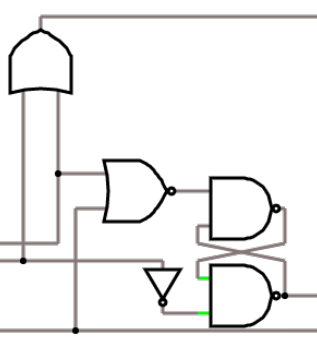
\includegraphics[scale=.5]{IM_SignBit}
    \caption{The component used to check a number sign, created with a flip-flop}
    \label{SignBit}
\end{figure}


\subsection{Memory}
The final part of the input is the two memories in figure \ref{Memories}.

\begin{figure}[h]
    \centering  
    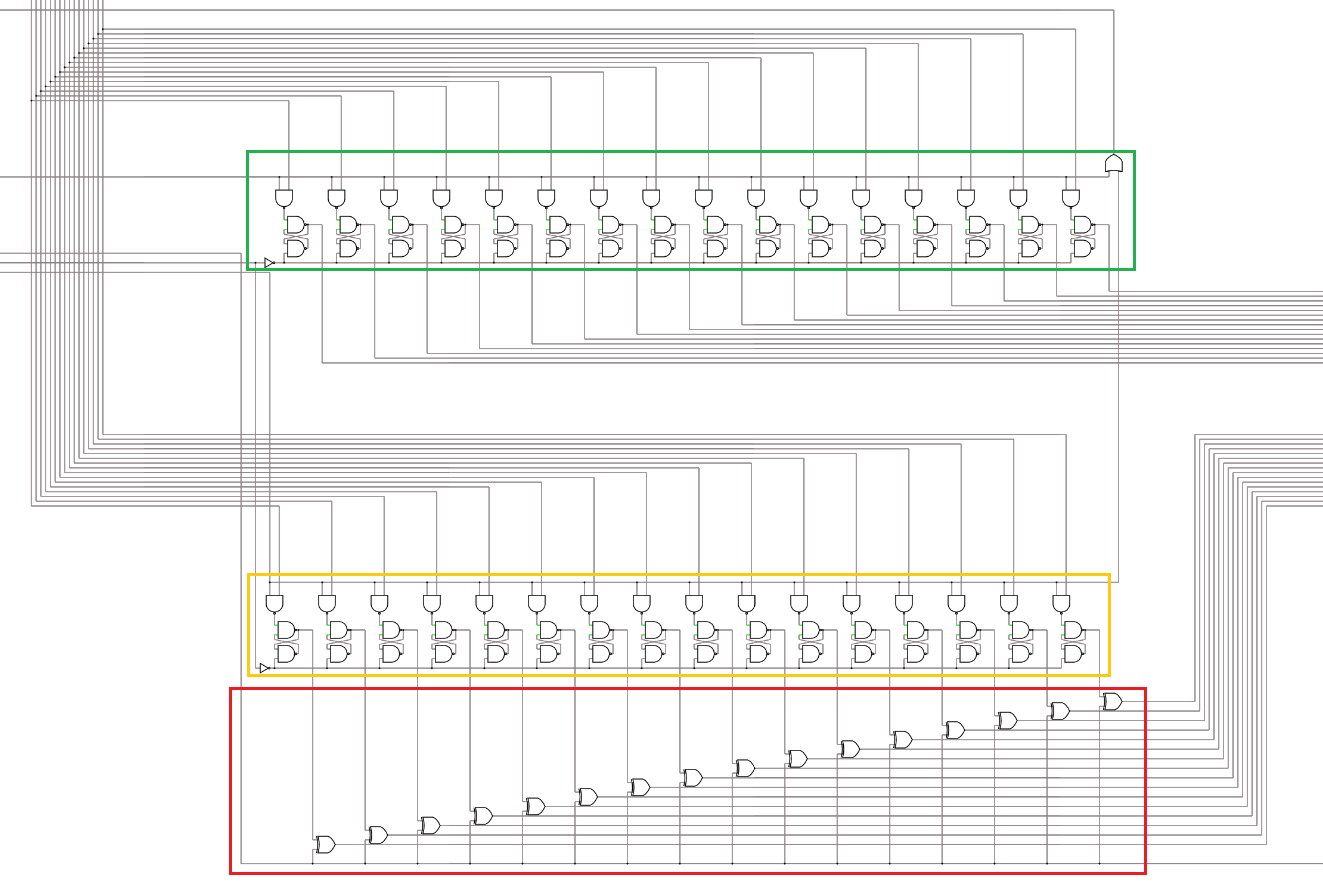
\includegraphics[scale=.4]{IM_Memories.PNG}
    \caption{Final part of the input section, composed by two memories, one for each number that needs storage}
    \label{Memories}
\end{figure}

\vspace{3mm}

The first memory, highlighted in green, is where the first number gets stored. Considering that the first number is always positive, we can save it, and give it to the processing section, just as it is. 

\vspace{1mm}

Since we want this memory to be modified only when it has to register the first number, we added the AND wire that is controlled by the wire exiting the OR in figure \ref{SignBit}. 

\vspace{1mm}

With this, the memory will store information only when $+$ or $-$ are pressed. The wire is also connected to the right,side of the memory to a line that clear the memory from immage%number of immage (10x multiplier)
making it possible to input the second number.

\vspace{3mm}

The second memory, highlighted in yellow, works in the same way as the first one but take the check at the input is done with the $=$ sign instead. %eh?

One difference between the first and second memory are the XOR gates beyond the second memory. A XOR takes as first input a bit and as second the sign bit. Then the XOR output will be the same as the first input if the sign bit is positive, and inverted if negative. This is done to perform an addition between a negative and a positive number. 

\vspace{3mm}

To see the complete process about the addition of positive and negative number check section \ref{DEVOMETTERLOZIO}

\subsection{Clear}

The last input, not discussed yet, is the clear button. This button is connected to the reset line of all the memories and the sign bit, and it switches every flip-flop to 0. 

\clearpage
\subsection{Decoder}

After the inputs have been processed (added or subtracted), it is needed a decoder (see figure \ref{Decoder}) in order to convert the output from binary number to its decimal form. Considering that this 16-bit calculator allows the user to insert numbers within the range (INSERIRE IL RANGE CAZZO), the operative boundary of this calculator is (INSERIRE).

\vspace{3mm}

The largest number that can be shown as result is around $\pm$INSERIER (+INSERIER or -INSERIER, to be exact), both positive and negative. So the decoding circuit needs to have 6 led displays for the digits and one extra display for the sign.

\vspace{3mm}

We decided to operate the binary-decimal conversion with the so called "double dabble" circuit, that will be explained later in the report. Nevertheless this was not the main problem. The double-dabble converts positive numbers perfectly, but not negative ones. The major issue was to adapt this circuit to work with both positive and negative numbers. 

The representation of the negative binary numbers follows the "two's complement" rule. It means that taken a B number of bits, all the numbers that can be represented with a 0 in the $B-1$ position are considered positive, otherwise they are negative. This allows to split the 17 bits available in two sets of 16 bits, and so it is possible to have the range described above.

\begin{figure}[h]
    \centering
    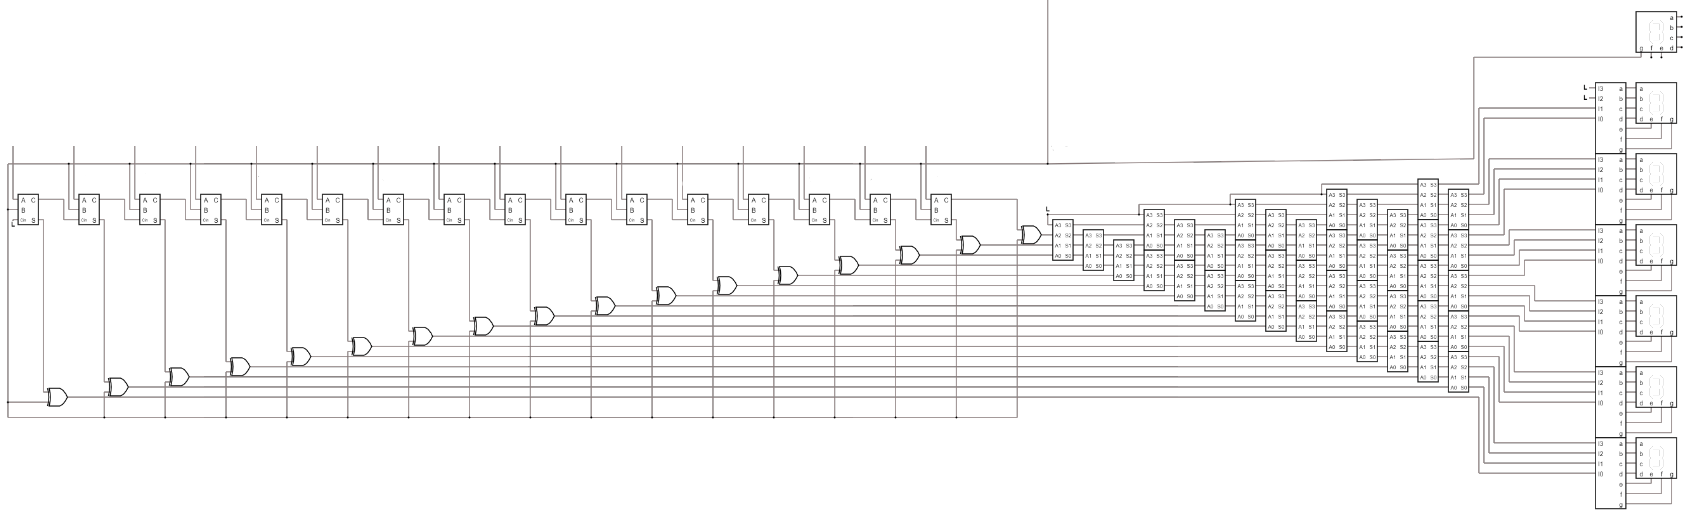
\includegraphics[scale=0.42]{SC_Decoder}
    \caption{Picture of the decoder}
    \label{Decoder}
  \end{figure}

\subsubsection{About the number sign}

The number sign has to be taken into account before converting the number into its decimal form. The number is a 16-bit binary, as already said, and it has one extra bit for the sign, the 16th bit.


This part of the circuit (represented in figure \ref{Converter}) uses full-adders and XOR logic gates, components that got already discussed in the previous sections. After the processing of the operation between the two inputs, the first 16 bits reach the A input of a specific full adder (the green lines in figure \ref{Converter}), whereas the sign bit follows the red path.

This 16th bit reaches every B input of all the full adders, and also the XOR gates, that compare the result of the single full adders with the 16th bit. The sign bit is true (or 1) when the number is negative and 0 otherwise. This allows the full adders to sum 1, following the formula above, if the processing output is negative, whereas if it is positive the number just stays the same.

After this, the XOR gates, which truth table is 
\begin{center}
\begin{tabular}{||c|c||c||}
    \hline
    A & B & A XOR B \\
    \hline
    0 & 0 & 0 \\
    \hline
    0 & 1 & 1 \\
    \hline
    1 & 0 & 1 \\
    \hline
    1 & 1 & 0 \\
    \hline
\end{tabular}
\end{center}

give the final result, which will go to the double dabble. Considering the full adder output as "A" for the XOR, and the sign bit as "B", it is possible to deduct that when the sign is false (so the processing output is positive) the XOR gates do not modify the full adder output (which do not work too, considering that their "B", the sign bit, is false as well). When the XOR "B" is true (so the processing output is negative), the XOR gives the opposite of its "A" as output.

\begin{figure}[h]
    \centering
    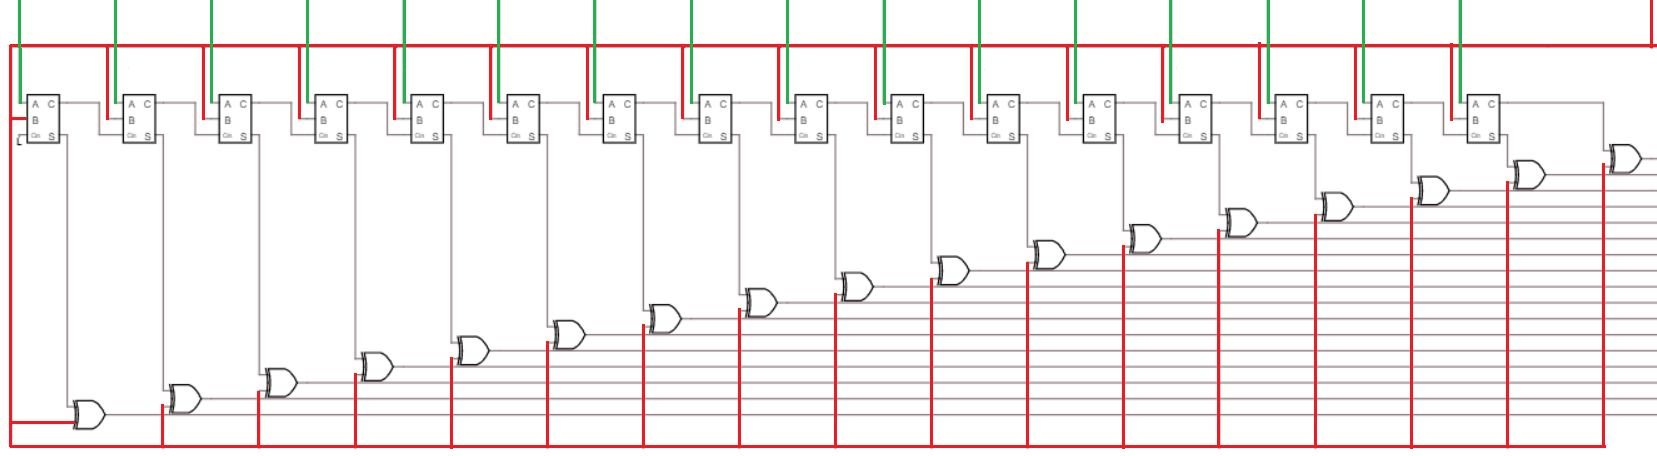
\includegraphics[scale=0.43]{SC_Converter.PNG}
    \caption{Picture of the first part of the decoder}
    \label{Converter}
  \end{figure}

\subsubsection{Double dabble}

This second part of the decoder is reached by the number that needs to be converted into decimal form. 

The entire circuit relies on an algorithmic process based on the concept of "shift and add 3", which is the name of the component that mostly populates figure \ref{DoubleDabble}.

This algorithm takes a binary number and after having processed it gives an output divided into smaller parts composed of 4 bits each. Everyone of these parts will be then elaborated by 7 segment decoders and represent a single digit of the decimal number. The 7-segment decoders are obviously connected to 7-segments led displays, that can be seen on the right side of figure \ref{DoubleDabble}.

\begin{figure}[h]
    \centering
    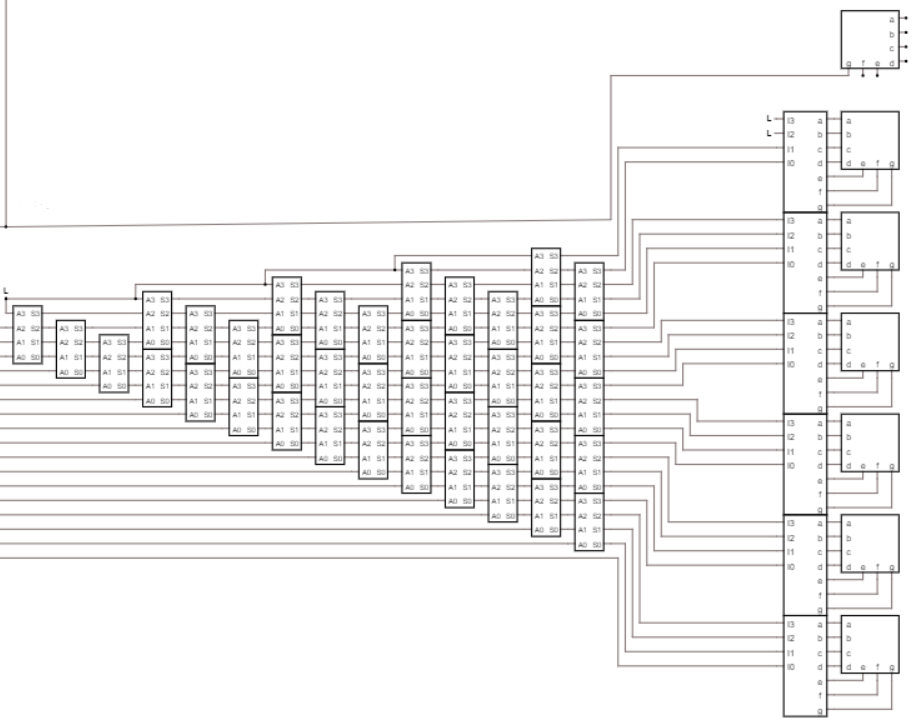
\includegraphics[scale=0.43]{SC_DoubleDabble}
    \caption{Picture of the double dabble, the second part of the circuit}
    \label{DoubleDabble}
  \end{figure}


The algorithm works as follows (graphic representation in figure \ref{SC_Algo}):
\begin{enumerate}
  \item Let's consider a 8-bit binary number, but the same argument works for n bits. 
  \item Let's consider the units, as long as that binary value is lower or equal to 4, the binary input can keep shifting and increasing the units.
  \item When the units value is an integer greater than 4, 3 is added to them and the shifting process continues.
\end{enumerate}

It is mandatory to add 3 because during the conversion the weight of the 4 bits of the unit is 16, at maximum, whereas those for digits represent a maximum of 10 in decimal form. So to compensate this loss, we add a half of the lost weight.

\begin{table}[h]
  \centering
  \begin{tabular}{||c|c|c|c||c||c||}
    \hline
    \# & Hundreds & Tens & Units & Binary & Operation \\
    \hline
    1 & 0000 & 0000 & 0000 & 11111111 & Start \\
    2 & 0000 & 0000 & 0001 & 11111110 & Shift1 (every 4-bit slot < 5) \\
    3 & 0000 & 0000 & 0011 & 11111100 & Shift2 (every 4-bit slot < 5) \\ 
    4 & 0000 & 0000 & 0111 & 11111000 & Shift3 (every 4-bit slot < 5) \\
    5 & 0000 & 0000 & 1010 & 11110000 & Add-3 to "Units" ("Units" $\geq$ 5)\\
    6 & 0000 & 0001 & 0101 & 11110000 & Shift4 (every 4-bit slot < 5) \\
    7 & 0000 & 0001 & 1000 & 11110000 & Add-3 to "Units" ("Units" $\geq$ 5)\\
    8 & 0000 & 0011 & 0001 & 11100000 & Shift5 (every 4-bit slot < 5) \\
    9 & 0000 & 0110 & 0011 & 11000000 & Shift6 (every 4-bit slot < 5) \\
    10 & 0000 & 1001 & 0011& 11000000 & Add-3 to "Tens" ("Tens" $\geq$ 5)\\
    11 & 0001 & 0010 & 0111& 10000000 & Shift7 (every 4-bit slot < 5) \\
    12 & 0001 & 0010 & 1010& 10000000 & Add-3 to "Units" ("Units" $\geq$ 5)\\
    13 & 0010 & 0101 & 0101& 00000000 & Shift8 (every 4-bit slot < 5) \\
    \hline
  \end{tabular}
    \label{SC_Algo}
    \caption{Double dabble algorithm applied to the decimal number 255}

  \end{table}


The goal of the "Shift and add 3" component, programmed using the customizable logic of the simulator, is to operate this shift or addition depending on the 4 inputs given. Its truth table is figure \ref{Add3Table}.

\begin{table}[h]
  \centering
  \begin{tabular}{||c|c||}
    \hline
    Input & Output \\
    \hline
    0000 & 0000 \\
    0001 & 0001 \\
    0010 & 0010 \\ 
    0011 & 0011 \\
    0100 & 0100 \\
    0101 & 1000 \\
    0110 & 1001 \\
    0111 & 1010 \\
    1000 & 1011 \\
    1001 & 1100 \\
    \hline
  \end{tabular}
    \label{Add3Table}
    \caption{"Shift and add 3" truth table}
  \end{table}

It is clear, thanks to this figure, that when the number is greater than four it gets added three to it. The "shift" part can be seen in figure \ref{DoubleDabble}. If we consider the input A0 of a single Add3 component, when can see that its output, S0, is the input A1 for the next component.

After all this process the number is divided into 4 bit groups that enter the 7-segment decoders and than display the result.






\clearpage
\section{Appendix}

\begin{figure}[h]
    \centering
    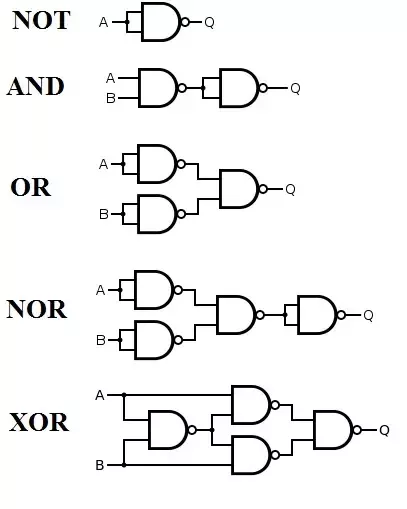
\includegraphics[scale=.42]{IM_NAND_allpowerful.png}
    \caption{NAND gate is functional complete, every other logic gate can be a circuit made of NANDs only}
    \label{NAND_allpowerful}
\end{figure}

\begin{figure}[h]
    \centering
    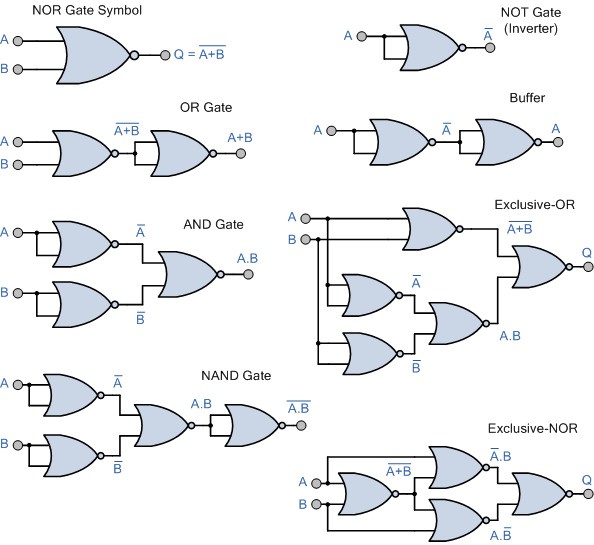
\includegraphics[scale=.5]{IM_NOR_allpowerful.png}
    \caption{NOR gate is functional complete, every other logic gate can be a circuit made of NORs only}
    \label{NOR_allpowerful}
\end{figure}

\end{document}